\subsection{Threshold}

Als image threshold wordt er gebruik gemaakt van de ISO data variant. Dit is een
automatische threshold die de juiste waarde bepaald vanuit het histogram. Hierbij
wordt uitgegaan van een 2-piek verdeling tussen de achtergrond en object pixels.
Hierbij wordt gezocht naar een \emph{valley} van het histogram.

\begin{figure}
    \begin{center}
        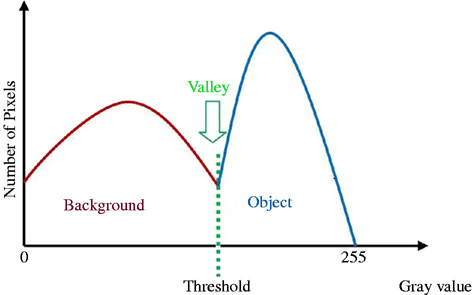
\includegraphics[scale=0.35]{figures/histogram.png}
    \end{center}
    \caption{Een 2-piek beeld verdeeld histogram}
    \label{fig:histogram}
\end{figure}

Vervolgens zal de functie van alle pixels boven/onder zijn threshold een 1 maken
en van alle pixels onder/boven zijn threshold een 0 maken.

De ISO data threshold gebruikt de 1ste pixel waarde en de som van alle pixels om
de threshold waarden te bepalen. Wiskundig kan dat als volgt uitgedrukt worden:

\[ Th = s + \frac{\sum\limits_{x=0}^{x_{max-1}} \sum\limits_{y=0}^{y_{max-1}} f(x, y)}{x_{max} y_{max}} \]

Waarbij $Th$ de threshold functie is en $s$ de start waarde van de pixels.

Door de som van alle pixels tegelijk te bepalen met het histogram is het
mogelijk om een threshold te volbrengen na 2 keer het hele plaatje te hebben
gescand.

In pseudo code zal dan de threshold waarde als volgt bepaald worden:

\begin{cppcode}
    for(i = 0; histogram[i] > 0; i++){
        continue;
    }

    Th = i + (sum / image_size);
\end{cppcode}

Daarna  kan er eenvoudig met een if-statement een threshold worden gedaan:

\begin{cppcode}
    if(data >= min && data <= max){
        data = 1;
    } else {
        data = 0;
    }
\end{cppcode}

Gezien de $x$ en $y$ waarden niet belangrijk zijn kan er het snelst door het
plaatje gegaan worden met behulp van een pointer.
